\chapter{Задача декодирования в пространстве высокой размерности}
\label{ch:pls}

В данной главе ставится формальная постановка задачи декодирования в терминах проекций в скрытое пространство. 
Вводятся понятия скрытого пространства, и процедура согласования образов.
Доказываются теоремы об оптимальном выборе модели декодирования.

\section{Формальная постановка задачи декодирования}

\hrulefill

Пусть имеется два множества временных рядов $\mathcal{S}^x = \{\bs^x_i\}_{i=1}^m$ и $\mathcal{S}^y = \{\bs^y_i\}_{i=1}^r$, состоящие из $m$ и $r$ временных рядов соответственно. 
Первое множество $\mathcal{S}^x$ является множеством временных рядов $m$ входных сигналов. 
Второе множество $\mathcal{S}^y$ является множеством временных рядов $r$ целевых сигналов.
Каждый временной ряд $\bs = (s_1, s_2, \dots, s_T)$ является последовательность измерений некоторый величины в течение времени. 
\begin{definition}
	Временное представление $\bx_t = ([\bs^x_1]_t, \dots, [\bs^x_m]_t) \in \bbR^m$ состоит из измерений временных рядов входных сигналов в момент времени $t$. 
	Аналогично временное представление $\by_t = ([\bs^y_1]_t, \dots, [\bs^y_r]_t) \in \bbR^r$ состоит из измерений временных рядов целевых сигналов в момент времени $t$.
\end{definition}
\begin{definition}
	Определим представление предыстории длины $h$ для момента времени $t$ множества временных рядов входных сигналов $\mathcal{S}^x$ как совокупность представлений $\bX_{t,h} = [\bx_{t - h + 1}, \dots, \bx_{t}]^{\T} \in \bbR^{h \times m}$.
	Аналогично определим представление предыстории длины $h$ для момента времени $t$ множества временных рядов целевых сигналов $\mathcal{S}^y$ как совокупность представлений $\bY_{t,h} = [\by_{t - h + 1}, \dots, \by_{t}]^{\T} \in \bbR^{h \times r}$.
\end{definition}
\begin{definition}
	Определим представление горизонта прогнозирования длины $p$ для момента времени $t$ множества временных рядов входных сигналов $\mathcal{S}^x$ как совокупность представлений $\bX_{t,p} = [\bx_{t + 1}, \dots, \bx_{t + p}]^{\T} \in \bbR^{p \times m}$.
	Аналогично определим представление горизонта прогнозирования длины $p$ для момента времени $t$ множества временных рядов целевых сигналов $\mathcal{S}^y$ как совокупность представлений $\bY_{t,r} = [\by_{t + 1}, \dots, \by_{t + p}]^{\T} \in \bbR^{p \times r}$.
\end{definition}

Задача авторегрессионного декодирования состоит в построении предсказательной модели $f_{\text{AR}}$, дающий прогноз представления горизонта прогнозирования множества временных рядов по представлению предыстории прогнозирования того же множества временных рядов.

\begin{definition}
	Предсказательная модель $f_{\text{AR}}^x: \bbR^{h \times m} \rightarrow \bbR^{p \times m}$ является авторегрессионной моделью, которая по представлению предыстории $\bX_{t,h}$ множества временных рядов входных сигналов $\mathcal{S}^x$ предсказывает представление горизонта прогнозирования $\bX_{t,p}$ множества временных рядов входных сигналов $\mathcal{S}^x$.
	Аналогично вводится предсказательная модель $f_{\text{AR}}^y: \bbR^{h \times r} \rightarrow \bbR^{p \times r}$ для множества целевых сигналов $\mathcal{S}^y$.
\end{definition}
Суть авторегрессионного декодирования заключается в предсказании будущего прогноза временного ряда по его же предыстории.

\begin{definition}
	Определим задачу регрессионного декодирования как задачу построения предсказательной модели $f_{\text{R}}^{xy}: \bbR^{h \times m} \rightarrow \bbR^{p \times r}$, которая по представлению предыстории $\bX_{t,h}$ множества временных рядов входных сигналов $\mathcal{S}^x$ предсказывает представление горизонта прогнозирования $\bY_{t,p}$ множества временных рядов целевых сигналов $\mathcal{S}^y$.
\end{definition}

Отличие регрессионного декодирования от авторегрессионного декодирования состоит в том, что в случае регрессионного декодирования представление предыстории и представление горизонта прогнозирозирования получены из временных рядов разных пространств, а именно предыстория получена из множества входных сигналов, в то время как горизонт прогнозирования получен из множества целевых сигналов.

\begin{definition}
	Общая задача декодирования состоит в построении предсказательной модели $f^{xy}: \bbR^{h_x \times m} \times \bbR^{h_y \times r} \rightarrow \bbR^{p \times r}$, которая по представлениям предыстории $\bX_{t,h_x}$ и $\bY_{t,h_y}$ временных рядов входных и целевых сигналов предсказывает представление горизонта прогнозирования $\bY_{t,r}$ временных рядов целевых сигналов. 
\end{definition}

Отметим, что авторегрессионная модель $f_{\text{AR}}^y$ и регрессионная модель $f_{\text{R}}^{xy}$ являются частными случаями общей задачи декодирования. А именно, авторегрессионная модель $f_{\text{AR}}^y$ соответствует случаю пустой предыстории временных рядов входных сигналов (случаю $h_x = 0$), а регрессионная модель $f_{\text{R}}^{xy}$ соответствует случаю пустого предыстории временных рядов целевых сигналов (случаю $h_y = 0$).

На Рис.~\ref{ch2:time_series_decoding} схематично продемонстрированы принципы построения введенных моделей декодирования временных рядов.

\begin{figure}
	\centering
	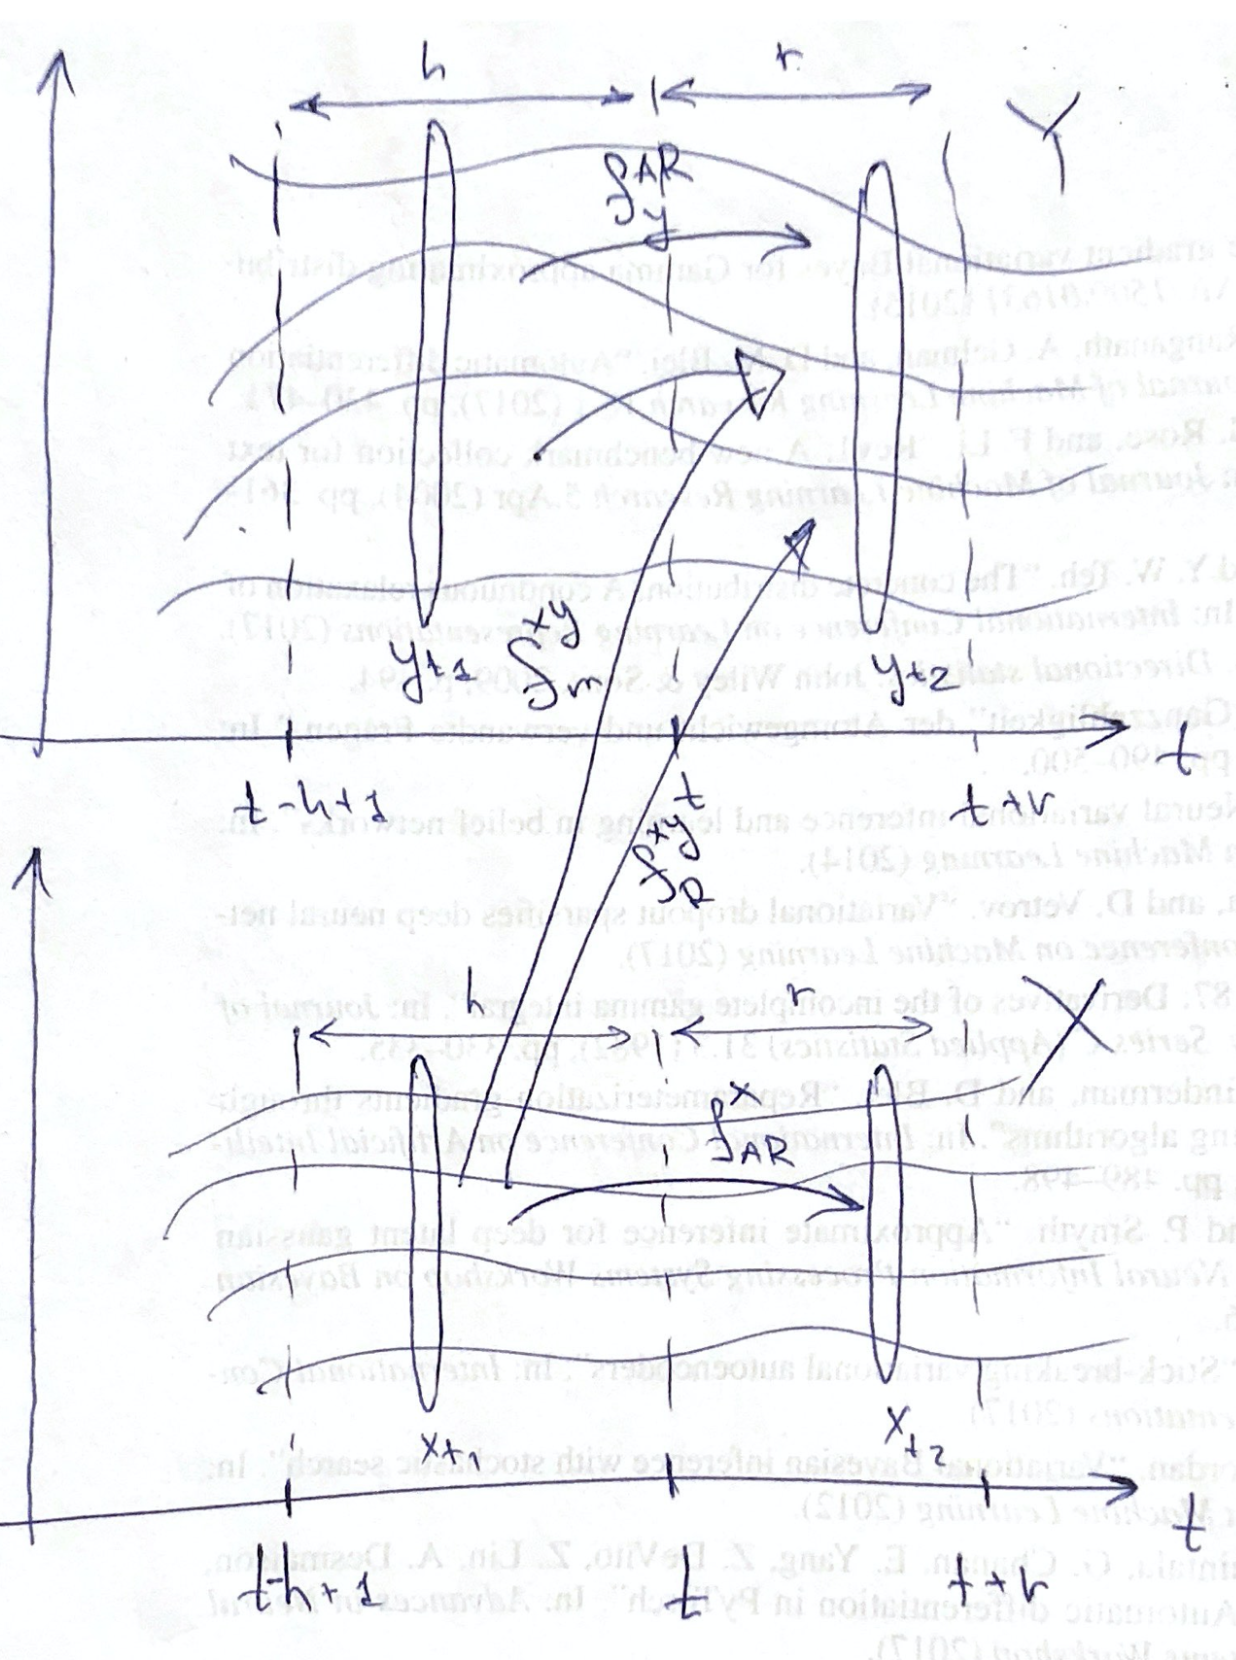
\includegraphics[width=0.5\linewidth]{figs/ch2/time_series_decoding}
	\caption{Схема построения моделей декодирования}
	\label{ch2:time_series_decoding}
\end{figure}

\begin{theorem}
	При определенных условиях (???) - [линейность моделей, уровень корреляции сигнала, обусловленность матрицы] предсказательная модель $f^{xy}: \bbR^{h_x \times m} \times \bbR^{h_y \times r} \rightarrow \bbR^{p \times r}$ лучше (???) - [меньше ошибка на трейн/вал, устойчивее решение, меньше размерность (простота)], чем авторегрессионная модель $f_{\text{AR}}^y$ и регрессионная модель $f_{\text{R}}^{xy}$.
\end{theorem}

\hrulefill

Для постановки задачи декодирования введём предположения о структурах пространств $\bbX$ и $\bbY$.
\begin{assumption}
	Рассмотрим случай, когда пространства $\bbX$ и $\bbY$ имеют избыточную размерность. 
	Это означает, что объекты $\bx$ и $\by$ принадлежат некоторым многообразиям низкой размерности. В простейшем случае такие многообразия могут являться вложениями, линейными подпространствами.
\end{assumption}

{\color{red} подумать, жирные ли буквы}

\begin{definition}
	Назовём пространство $\bbT \subset \bbR^l$ \textit{скрытым пространством} для пространства $\bbX \in \bbR^n$ ($l \leq n$), если существуют функция $\varphi_e: \bbX \to \bbT$ и функция $\varphi_d: \bbT  \to \bbX$ такие что
	\[
	\bx \in \bbX \quad \exists \bt \in \bbT: \varphi_d (\varphi_e(\bx)) = \varphi_d(\bt) = \bx.
	\]
	Функция $\varphi_e(\bx)$ называется \textit{функцией кодирования} объекта $\bx$, функция $\varphi_d(\bt)$  называется \textit{функцией декодирования}. 
	
	Аналогично введём определение \textit{скрытого пространства}~$\bbU \subset \bbR^s$ для целевого пространства $\bbY$, \textit{функции кодирования} $\psi_e: \bbY \to \bbU$ и \textit{декодирования} $\psi_d: \bbU  \to \bbY$
	\[
	 \by \in \bbY \quad  \exists \bu \in \bbU: \psi_d (\psi_e(\by)) = \psi_d(\bu) = \by.
	\]
\end{definition}

\begin{definition}
	Пространство $\bbT \subset \bbR^l$ задаёт \textit{внутреннюю структуру} пространства $\bbX \in \bbR^n$, если пространство $\bbT$ является скрытым для пространства $\bbX$.
\end{definition}

\begin{definition}
	Между пространствами $\bbX$ и $\bbY$ существует \textit{согласующее отображение}, если существуют пространства $\bbT$ и $\bbU$, задающие внутренние структуры для пространств $\bbX$ и $\bbY$ соответственно, и существует \textit{функция согласования} $g: \bbT \rightarrow \bbU$, такая что
	\[
	\bu \in \bbU \quad \exists \bt:  \bu = g(\bt).
	\]
\end{definition}

\begin{assumption}
	Предположим, что в задаче предсказания~\eqref{ch1:eq:loss_min} пространства $\bbT$ и $\bbU$ задают внутреннюю структуру пространств $\bbX$ и $\bbY$. 
	Предположим также, что для данных скрытых пространств $\bbT$ и $\bbU$ существует функция согласования~$g: \bbT \rightarrow \bbU$. Тогда выполнено
	\[
	\forall \by \in \bbY \quad \exists \bx \in \bbX: \by = \psi_d(\bu) = \psi_d(g(\bt)) = \psi_d(g(\phi_e(\bx))),
	\]
	и общая схема задачи декодирования принимает вид следующей коммутативной диаграммы:
	\begin{equation}
		\begin{tikzpicture}
			\matrix (m) [matrix of math nodes,row sep=3em,column sep=4em,minimum width=2em]
			{
				\bbX \subset \bbR^n & \bbY \subset \bbR^r \\
				\bbT \subset \bbR^l & \bbU \subset \bbR^s \\};
			\path[-stealth]
			(m-1-1) edge node [above] {$f$} (m-1-2)
			(m-2-1) edge [bend right=10] node [right] {$\varphi_d$} (m-1-1)
			(m-2-2) edge [bend left=10] node [left] {$\psi_d$} (m-1-2)
			(m-1-1) edge [bend right=10] node [left] {$\varphi_e$} (m-2-1)
			(m-1-2) edge [bend left=10] node [right] {$\psi_e$} (m-2-2)
			(m-2-1) edge node [above] {$h$} (m-2-2);
		\end{tikzpicture}
		\label{ch1:eq:decoding_scheme}
	\end{equation}


\begin{equation}
	\begin{tikzpicture}
		\matrix (m) [matrix of math nodes,row sep=3em,column sep=2em,minimum width=2em]
		{
			\bX \subset \bbR^n & & \bY \subset \bbR^r \\
			& \bT, \bU \subset \bbR^l & \\};
		\path[-stealth]
		(m-1-1) edge node [above] {$\mathbf{f}$} (m-1-3)
		(m-1-1) edge node [left=5] {$\bP$} (m-2-2)
		(m-1-3) edge node [right=5] {$\bQ$} (m-2-2);
	\end{tikzpicture}
\end{equation}
\end{assumption}

\begin{definition}
	Согласно диаграмме~\eqref{ch1:eq:decoding_scheme}, определим модель декодирования $f: \bbX \rightarrow \bbY$ как суперпозицию
	\begin{equation}
		f = \psi_d \circ g \circ \varphi_e.
		\label{ch1:eq:def_decoding_function}
	\end{equation}
\end{definition}

\section{Доказательство корректности работы алгоритмов PLS и CCA}

Псевдокод метода регрессии PLS приведен в Алгоритме~\ref{ch1:pls_pseudocode}.
Алгоритм итеративно на каждом из $l$ шагов вычисляет по одному столбцу $\bt_k$, $\bu_k$, $\bp_k$, $\bq_k$ матриц $\bT$, $\bU$, $\bP$, $\bQ$ соответственно. 
После вычисления следующего набора векторов из матриц $\bX$, $\bY$ вычитаются очередные одноранговые аппроксимации. 
При этом предполагается, что исходные матрицы~$\bX$ и~$\bY$ нормированы (имеют нулевое среднее и единичное среднее отклонение).

\begin{algorithm}[h]
	\caption{Алгоритм PLS}
	\label{ch1:pls_pseudocode}
	\begin{algorithmic}[1]
		\REQUIRE $\bX, \bY, l$;
		\ENSURE $\bT, \bP, \bQ$;
		\STATE нормировать матрицы $\bX$ и $\bY$ по столбцам
		\STATE инициализировать $\bu_0$ (первый столбец матрицы $\bY$)
		\STATE $\bX_1 = \bX; \bY_1 = \bY$
		\FOR{$k=1,\dots, l$}
		\REPEAT
		\vspace{0.1cm}
		\STATE $\bw_k := \bX_k^{\T} \bu_{k-1} / (\bu_{k-1}^{\T} \bu_{k-1}); \quad \bw_k: = \frac{\bw_k}{\| \bw_k \|}$
		\vspace{0.1cm}
		\STATE $\bt_k := \bX_k \bw_k$
		\vspace{0.1cm}
		\STATE $\bc_k := \bY_k^{\T} \bt_k / (\bt_k^{\T} \bt_k); \quad \bc_k: = \frac{\bc_k}{\| \bc_k \|}$
		\vspace{0.1cm}
		\STATE $\bu_k := \bY_k \bc_k$
		\UNTIL{$\bt_k$ не стабилизируется}
		\vspace{0.1cm}
		\STATE $\bp_k:= \bX_k^{\T}\bt_k/(\bt_k^{\T}\bt_k),\ 
		\bq_k := \bY_k^{\T}\bt_k/(\bt_k^{\T}\bt_k)$
		\vspace{0.2cm}
		\STATE $\bX_{k+1} :=  \bX_k - \bt_k \bp_k^{\T}$
		\vspace{0.2cm}
		\STATE $\bY_{k + 1} :=  \bY_k - \bt_k \bq_k^{\T}$ 
		\ENDFOR
	\end{algorithmic}
\end{algorithm}

Вектора $\bt_k$ и $\bu_k$ из внутреннего цикла Алгоритма~\ref{ch1:pls_pseudocode}
содержат информацию о матрице объектов $\bX$ и матрице ответов $\bY$ соответственно. 
Блоки из шагов (6)--(7) и шагов (8)--(9)~--- аналоги алгоритма PCA для матриц $\bX$ и $\bY$~\cite{geladi1988pls}. 
Последовательное выполнение блоков позволяет учесть взаимную связь между матрицами $\bX$ и $\bY$.

Теоретическое обоснование алгоритма PLS следует из следующих утверждений.
\begin{statement}
	Максимизации ковариации между векторами $\bt_k$ и $\bu_k$ сохраняет дисперсию столбцов матриц~$\bX$ и~$\bY$ и учитывает их линейную зависимость.
\end{statement}
\begin{proof}
	Утверждение следует из равенства
	\[
	\text{cov} (\bt_k, \bu_k) = \text{corr} (\bt_k, \bu_k) \cdot \sqrt{\text{var}(\bt_k)} \cdot \sqrt{\text{var}(\bu_k)}.
	\]
	Максимизация дисперсий векторов $\bt_k$ и $\bu_k$ отвечает за сохранение информации об исходных матрицах, 
	корреляция между векторами отвечает взаимосвязи между $\bX$ и~$\bY$. 
\end{proof}

Во внутреннем цикле Алгоритма~\ref{ch1:pls_pseudocode} вычисляются нормированные вектора весов $\bw_k$ и $\bc_k$. 
Из данных векторов строятся матрицы весов $\bW$ и $\bC$ соответственно.

\begin{statement}
	В результате выполнения внутреннего цикла вектора $\bw_k$ и $\bc_k$ будут собственными векторами матриц $\bX_k^{\T} \bY_k \bY_k^{\T} \bX_k$ и $\bY_k^{\T} \bX_k \bX_k^{\T} \bY_k$, соответствующими максимальным собственным значениям.
	
	\begin{equation*}
		\bw_k \varpropto \bX_k^{\T} \bu_{k-1} \varpropto \bX_k^{\T} \bY_k \bc_{k-1} \varpropto \bX_k^{\T} \bY_k \bY_k^{\T} \bt_{k-1} \varpropto \bX_k^{\T} \bY_k \bY_k^{\T} \bX_k \bw_{k-1},
	\end{equation*}
	\begin{equation*}
		\bc_k \varpropto \bY_k^{\T} \bt_k \varpropto \bY_k^{\T} \bX_k \bw_k \varpropto \bY_k^{\T} \bX_k \bX_k^{\T} \bu_{k-1} \varpropto \bY_k^{\T} \bX_k \bX_k^{\T} \bY_k \bc_{k-1},
	\end{equation*}
	где символ $\varpropto$ означает равенство с точностью до мультипликативной константы. 
	\label{st:eig}
\end{statement}
\begin{proof}
	Утверждение следует из того факта, что правила обновления векторов $\bw_k$, $\bc_k$ совпадают с итерацией алгоритма поиска максимального собственного значения. 
	Данный алгоритм основан на следующем факте.
	Если матрица $\mathbf{A}$ диагонализуема, $\bx$~--- некоторый вектор, то
	
	\[
	\lim_{k \rightarrow \infty} \mathbf{A}^k \bx = \lambda_{\max}(\mathbf{A}) \cdot \mathbf{v}_{\max},
	\]
	где $ \lambda_{\max} (\mathbf{A})$~--- максимальное собственное значение матрицы $\mathbf{A}$, $\mathbf{v}_{\max}$~---собственный вектор матрицы $\mathbf{A}$, соответствующий~$\lambda_{\max} (\mathbf{A})$.
	
\end{proof}

\begin{statement}
	Обновление векторов по шагам (6)--(9) Алгоритма~\ref{ch1:pls_pseudocode} соответствует максимизации ковариации между векторами~$\bt_k$ и~$\bu_k$.
\end{statement}
\begin{proof}
	Максимальная ковариация между векторами~$\bt_k$ и~$\bu_k$ равна максимальному собственному значению матрицы~$\bX_k^{\T} \bY_k \bY_k^{\T} \bX_k$:
	\begin{align*}
		\max_{\bt_k, \bu_k}  \text{cov} (\bt_k, \bu_k)^2 &= \max_{\substack{\|\bw_k\|=1 \\ \|\bc_k\| = 1}} \text{cov} \left( \bX_k \bw_k, \bY_k \bc_k \right)^2 = \max_{\substack{\|\bw_k\|=1 \\ \|\bc_k\| = 1}} \text{cov} \left(\bc_k^{\T}  \bY_k^{\T} \bX_k \bw_k \right)^2 = \\
		&= \max_{\|\bw_k\| = 1} \text{cov} \left\|\bY_k^{\T} \bX_k \bw_k \right\|^2 = \max_{\|\bw_k\| = 1} \bw_k^{\T} \bX_k^{\T} \bY_k \bY_k^{\T} \bX_k \bw_k = \\
		& = \lambda_{\max} \left( \bX_k^{\T} \bY_k \bY_k^{\T} \bX_k \right),
	\end{align*}
	где~$\lambda_{\max} (\mathbf{A})$~--- максимальное собственное значение матрицы $\mathbf{A}$.
	Применяя утверждение~\ref{st:eig}, получаем требуемое.
\end{proof}

После завершения внутреннего цикла на шаге (11) вычисляются вектора $\bp_k$, $\bq_k$ проецированием столбцов матриц $\bX_k$ и $\bY_k$ на вектор $\bt_k$. 
Для перехода на следующий шаг необходимо вычесть из матриц $\bX_k$ и $\bY_k$ одноранговые аппроксимации $\bt_k \bp_k^{\T}$ и $\bt_k \bq_k^{\T}$
\begin{equation*}
	\bX_{k + 1} = \bX_{k} - \bt_k \bp_k^{\T} = \bX - \sum_k \bt_k \bp_k^{\T},
\end{equation*}
\begin{equation*}
	\bY_{k + 1} = \bY_{k} - \bt_k \bq_k^{\T} = \bY - \sum_k \bt_k \bq_k^{\T}.
\end{equation*}
При этом каждый следующий вектор~$\bt_k$ оказывается ортогонален всем векторам~$\bt_i$, $i=1, \dots, k$.

Для получения прогнозов модели и нахождения параметров модели 
домножим справа формулу~\eqref{ch1:eq:PLS_X} на матрицу $\bW$. Строки матрицы невязок $\bE$ ортогональны столбцам матрицы $\bW$, поэтому 
\[
\bX \bW = \bT \bP^{\T} \bW.
\] 

Линейное преобразование между объектами в исходном и латентном пространстве имеет вид
\begin{equation}
	\bT = \bX \bW^*,
	\label{ch1:eq:W*}
\end{equation}
где $\bW^* = \bW (\bP^{\T} \bW)^{-1}$. 

Матрица параметров модели~\ref{ch1:eq:lin_reg_model} находится из уравнений~\eqref{ch1:eq:PLS_Y},~\eqref{ch1:eq:W*}
\begin{equation*}
	\bY = \bT \bQ^{\T} + \bE = \bX \bW^* \bQ^{\T} + \bE = \bX \bTheta + \bE.
	\label{ch1:eq:pls_model}
\end{equation*}
Таким образом, параметры модели~\eqref{ch1:eq:lin_reg_model} равны
\begin{equation}
	\bTheta = \bW (\bP^{\T} \bW)^{-1} \bQ^{\T}.
	\label{ch1:eq:linear_regression_model_parameters}
\end{equation}

Финальная модель~\eqref{ch1:eq:pls_model} является линейной, низкоразмерной в скрытом пространстве. 
Это снижает избыточность данных и повышает стабильность модели.

\hrulefill

\textbf{Алгоритмы PCA, PLS, CCA, DeepCCA в терминах задачи декодирования (работа Фаруха)}

\begin{figure}[!ht]
	\centering
	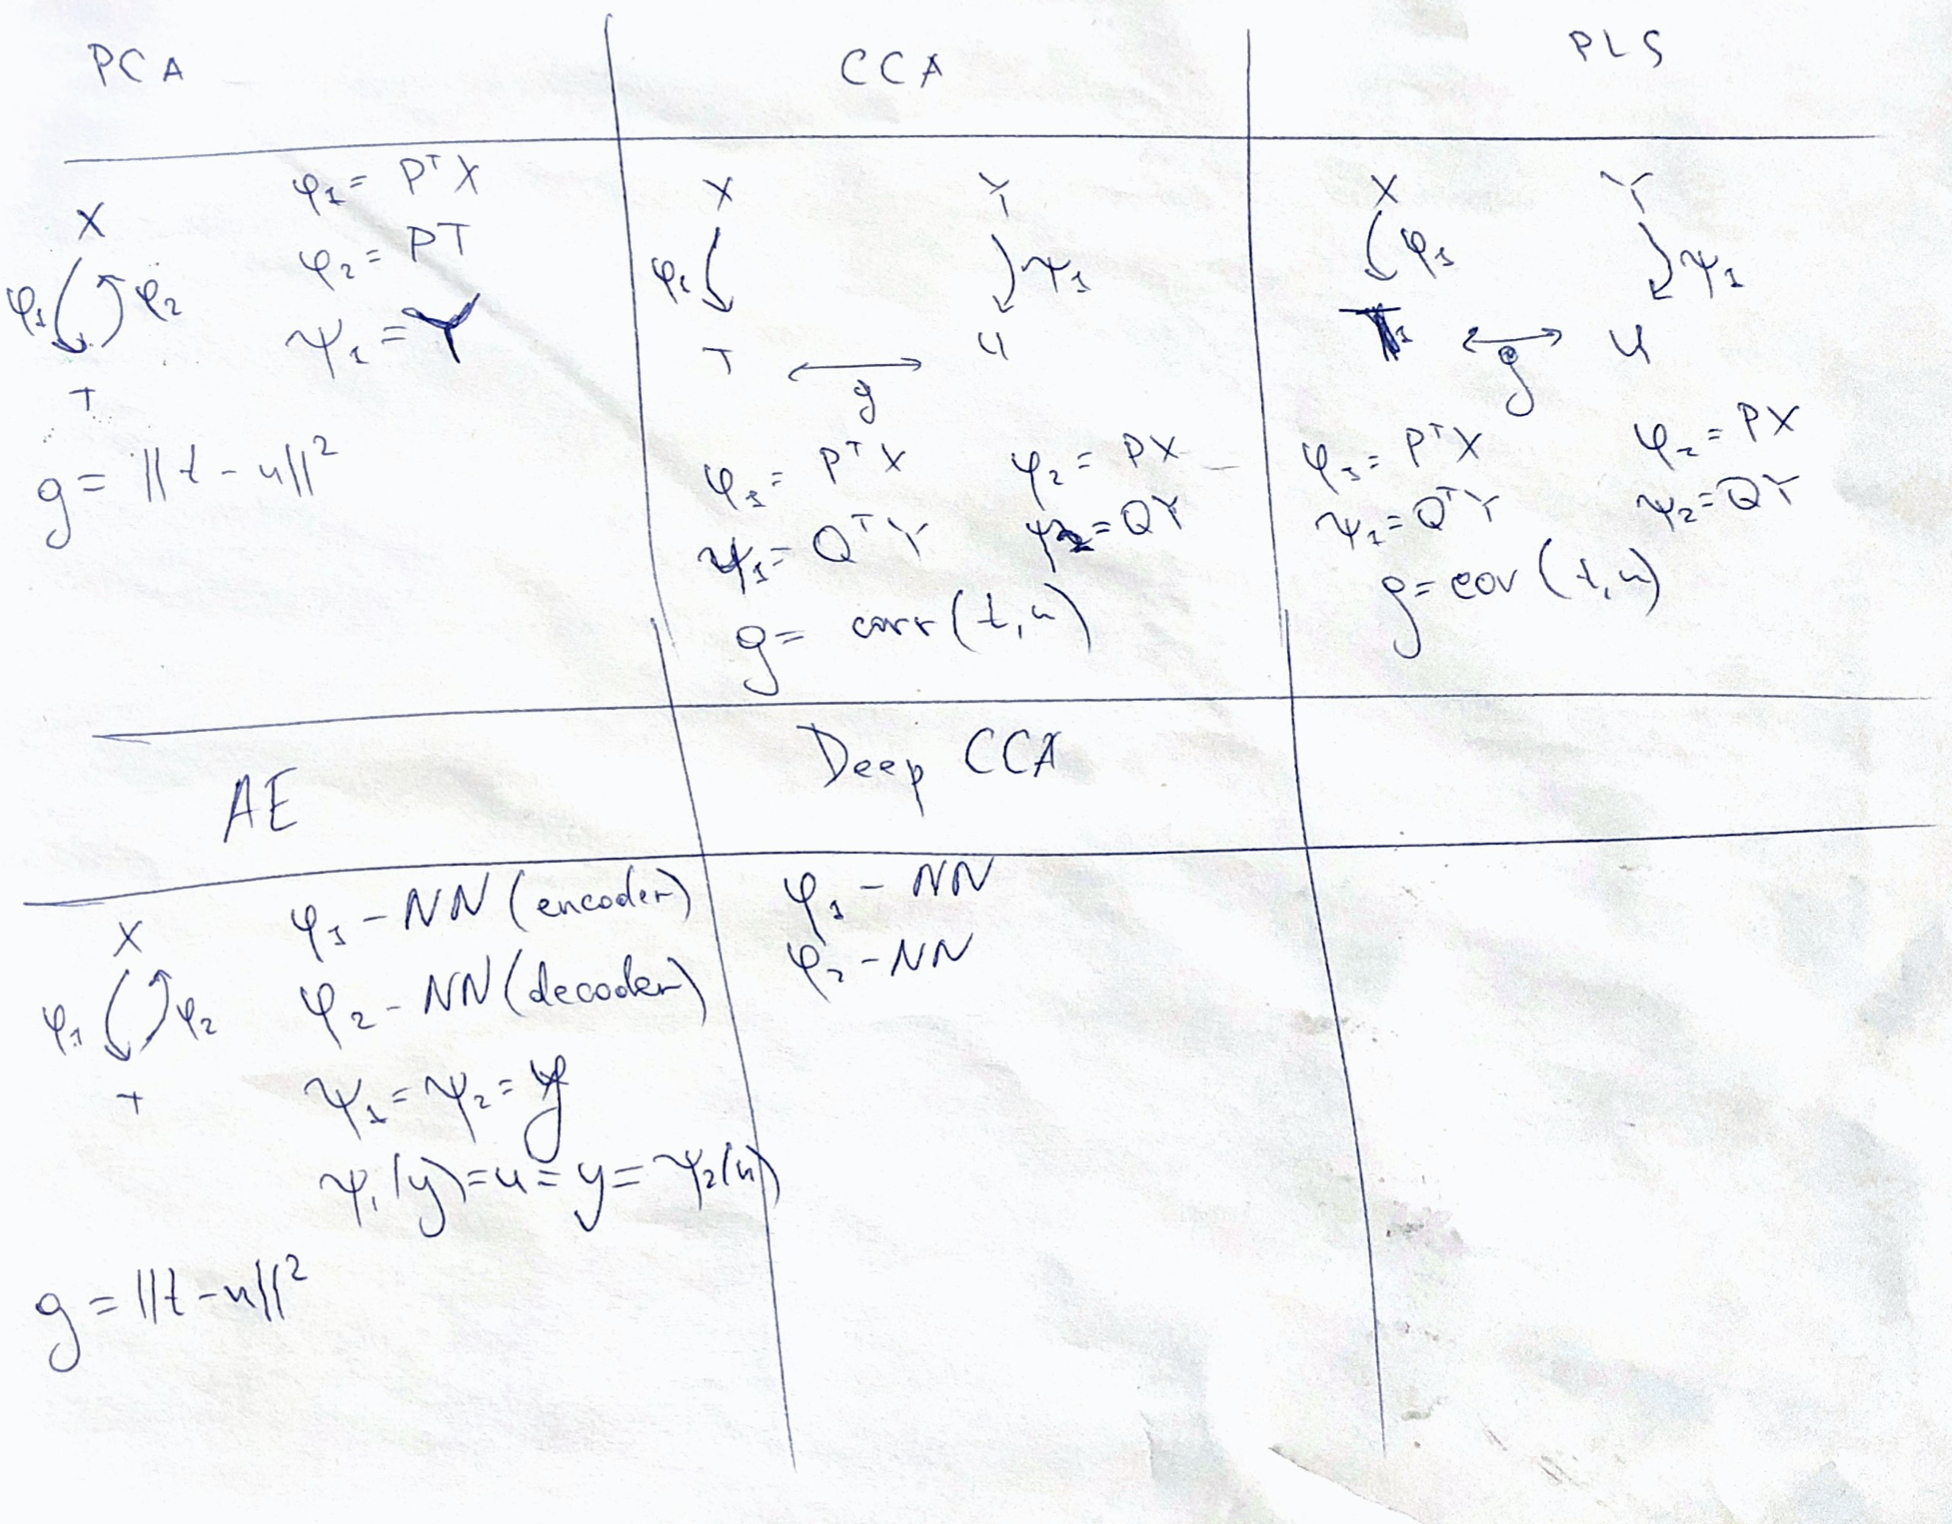
\includegraphics[width=\linewidth]{figs/ch1/Examples}
	\caption{Примеры алгоритмов, работающих по схеме \ref{ch1:eq:decoding_scheme}}
	\label{ch1:fig:PLSFigure}
\end{figure}

\begin{definition}
Параметрическая функция $\varphi_1: \mathbb{R}^{n \times m} \to \mathbb{R}^{n \times p}$, переводящая исходные данные в латентное пространство, называется \textbf{функцией кодирования}.
\end{definition}

\begin{definition}
	Функция $\varphi_2: \mathbb{R}^{n \times p} \to \mathbb{R}^{n \times m}$, переводящая данные из латентного пространства в исходное, называется \textbf{функцией восстановления}.
\end{definition}

\begin{definition}
	Функция $g: \mathbb{R}^{n \times p}\times \mathbb{R}^{n \times p} \to \mathbb{R}$, связывающая закономерности в низкоразмерных латентных представлениях, называется \textbf{функцией согласования}.
\end{definition}

\begin{definition}
	Согласование~--- алгоритмическая процедура максимизации функции согласования.
\end{definition}

Коммутативная диаграмма процедуры выбора прогностической модели имеет вид
\begin{equation}
\begin{tikzpicture}
	\matrix (m) [matrix of math nodes,row sep=3em,column sep=4em,minimum width=2em]
{
	\underset{n \times m}{\bX} & \underset{n \times k}{\bY} \\
	\underset{n \times p}{\mathbf{T}} &  \underset{n \times p}{\mathbf{U}} \\};
	\path[-stealth]
	(m-2-1) edge node [right] {$\varphi_2$} (m-1-1)
	(m-2-2) edge node [left] {$\psi_2$} (m-1-2)
	(m-1-1) edge [bend right] node [left] {$\varphi_1$} (m-2-1)
	(m-1-2) edge [bend left] node [right] {$\psi_1$} (m-2-2)
	(m-2-1) edge [<->] node [above] {$g$} (m-2-2)
	(m-1-1) edge [->] node [above] {$f$} (m-1-2);
\end{tikzpicture}
\label{eq:scheme}
\end{equation}
где $\varphi_1: \mathbb{R}^{n \times m} \to \mathbb{R}^{n \times p}$~---  функция кодирования независимых переменных; $\psi_1: \mathbb{R}^{n \times k} \to \mathbb{R}^{n \times p}$~---  функция кодирования целевых переменных; $\varphi_2: \mathbb{R}^{n \times p} \to \mathbb{R}^{n \times m}$~---  функция восстановления независимых переменных; $\psi_2: \mathbb{R}^{n \times p} \to \mathbb{R}^{n \times k}$~--  функция восстановления целевых переменных; $g: \mathbb{R}^{n \times p} \times \mathbb{R}^{n \times p} \to \mathbb{R}$~--- функция согласования.
Матрицы
\[
	\bT = \varphi_1(\bX)  \in \mathbb{R}^{n\times p}; \quad \bU =\psi_1(\bY) \in \mathbb{R}^{n\times p}
\]
являются матрицами представлений данных в латентном пространстве низкой размерности.

Оптимальные параметры $\theta_{\varphi_1}^{*}, \theta_{\psi_1}^{*}$ для функций кодирования $\varphi_1$  и $\psi_1$ находятся из следующей задачи параметрической оптимизации:
\begin{equation}
	(\theta_{\varphi_1}^{*}, \theta_{\psi_1}^{*}) = \argmax_{(\theta_{\varphi_1}, \theta_{\psi_1})} g\bigl( \varphi_1(\bX; \theta_{\varphi_1}), \psi_1(\bY; \theta_{\psi_1})\bigr).
\label{eq:argmax}
\end{equation}

Так как параметры функции кодирования подбираются из условия максимизации функции согласования~\eqref{eq:argmax}, то после перехода в латентное пространство между $\mathbf{T}$ и $\mathbf{U}$ существует зависимость
\begin{equation}
	\bU = h(\bT) +  \boldsymbol{\eta},
	\label{eq:reg2}
\end{equation}
где $h: \mathbb{R}^{n \times p} \to \mathbb{R}^{n \times p}$~--- функция регрессионной зависимости,  $\boldsymbol{\eta}$~--- матрица регрессионных ошибок.
Оптимальная функция $h$ выбирается минимизацией функции ошибки. Используется квадратичная функция потерь $\mathcal{L}$ на $\bT$ и $\bU$:
\begin{equation}
	\mathcal{L}(h | {\bT}, {\bU}) = {\left\| \underset{n \times p}{\bU}  - h(\underset{m \times p}{\bT}) \right\| }_2^2 \rightarrow\min_{h}.
	\label{eq:loss_function}
\end{equation}

Финальная прогностическая модель имеет вид
$\widehat{\by} = \psi_2\bigl(h(\varphi_1(\bx))\bigr)$, то есть

\begin{equation}
	f = \psi_2 \circ h \circ \varphi_1.
	\label{eq:f}
\end{equation}

Метод главных компонент (PCA) снижает размерность данных и сохраняет максимальную дисперсию. Линейная модель PCA представляет собой ортогональное линейное преобразование исходного признакового пространства в новое пространство меньшей размерности. Первый базисный вектор строится так, чтобы выборочная дисперсия столбцов проекций матрицы~$\bX$ была максимальной:
\begin{equation}
	\bp = \argmax_{\|\bp\|_{2} = 1} [\textbf{var}(\bX \textbf{p})],
	\label{eq:PCA}
\end{equation}
где $\textbf{var}(\bX \textbf{p}) = \frac{1}{n} (\bX \textbf{p})^{\T}\bX \textbf{p}$ обозначает выборочную дисперсию. Последующие базисные векторы находятся итеративно после вычитания проекции на все найденные ранее.

Функция кодирования $\varphi_1: \mathbb{R}^{n \times m} \to \mathbb{R}^{n \times p}$ имеет вид
\begin{equation}
	\varphi_1(\bX) =  \underset{n \times m}\bX \cdot \underset{m \times p}\bP^{\T},
	\label{eq:PCA2}
\end{equation}
где $\textbf{P} = [\textbf{p}_1, \dots, \textbf{p}_{p}].$
Метод PCA не согласует независимые переменные и целевые переменные. Из-за этого зависимости в обоих пространствах не учитываются.


Метод частичных наименьших квадратов восстанавливает связь между двумя наборами данных $\bX$ и $\bY$. Алгоритм проецирует $\bX$ и $\bY$ на латентное пространство $\mathbb{R}^{p}$ меньшей размерности. PLS находит матрицы исходных данных $\bX$ и $\bY$ в латентном пространстве $\textbf{T}$ и $\textbf{U}$ соответственно. Матрица объектов $\bX$ и целевая матрица $\bY$ проецируются на латентное пространство следующим образом:
\begin{align}
	\underset{n \times m}{\bX}  &= \underset{n \times p}{\textbf{T}} \cdot \underset{p \times m}{\textbf{P}}^{\T} +  \underset{n \times m}{\textbf{F}},
	\label{eq:PLSpr1} \\
	\underset{n \times k}{\bY}  &= \underset{n \times p}{\textbf{U}} \cdot \underset{p \times k}{\bQ}^{\T} + \underset{n \times k}{\textbf{E}},
	\label{eq:PLSpr2}
\end{align}
где $\textbf{T}$ и $\textbf{U}$~--- матрицы описания объектов и исходов в латентном пространстве; $\textbf{P}$ и $\textbf{Q}$~--- матрицы перехода из латентного пространства в исходное; $\textbf{F}$, $\textbf{E}$~--- матрицы остатков.

В методе PLS  функции кодирования имеют вид
\begin{equation*}
	\varphi_1(\bX) = \bX \bW_{\bx}, \;\;
	\psi_1(\bY) = \bY \bW_{\by},
\end{equation*}
где матрицы весов $\bW_{\bx} \in \mathbb{R}^{m \times p}, \bW_{\by} \in \mathbb{R}^{k \times p}$ находятся путем максимизации функции согласования $g(\bX \bW_{\bx},  \bY \bW_{\by}) = \textbf{Cov} (\bX \bW_{\bx},  \bY \bW_{\by})^{2}$:
\begin{equation}
	(\bW_{\bx}, \bW_{\by}) = \argmax_{\bW_{\by}, \bW_{\by}}[ \textbf{Cov}(\bX \bW_{\bx}, \bY \bW_{\by})^{2}],
\label{eq:PLSpr3}
\end{equation}
где $\textbf{Cov}(\bX \bW_{\bx}, \bY \bW_{\by})$~--- выборочная ковариация.

Функции восстановления принимают вид
\begin{equation*}
	\varphi_2(\bT) = \bT\bP^{\T}, \;\;
	\psi_2(\bU) = \bU \bQ^{\T}.
\end{equation*}

Канонический анализ корреляций находит два набора базисных векторов $\{\bw_{\bx_i}\}_{i=1}^{p}$, $\bw_{\bx} \in \mathbb{R}^{m}$, и $\{\bw_{\by_i}\}_{i=1}^{p}, \; \bw_{\by} \in \mathbb{R}^{k}$, один для матрицы $\bX$, другой для матрицы $\bY$, так чтобы коэффициент корреляция между проекциями переменных на эти базисные векторы был максимальным. Функция согласования для CCA имеет вид
\begin{equation*}
	g(\bX \bW_{\bx}, \bY \bW_{\by}) = \textbf{corr}(\bX \bW_{\bx}, \bY \bW_{\by}),
\end{equation*}
\noindentгде $\textbf{corr}(\bX \bw_{\bx}, \bY \bw_{\by})$~-- коэффициент корреляции между векторами.

Таким образом, функции кодирования имеют вид
\begin{equation*}
	\varphi_1(\bX) = \bX \bW_{\bx} , \;\;
	\psi_1(\bY) = \bY \bW_{\by},
\end{equation*}
где первые столбцы матриц весов находятся как векторы, максимизирующие функцию согласования $g$. Далее ищутся векторы, максимизирующие $g$, но с ограничением, что они не коррелируют с первой парой векторов. Процедура продолжается до тех пор, пока число векторов не станет равным $p$.

\textbf{Нелинейный канонический анализ корреляций}

Нелинейный канонический анализ корреляций~--- нелинейная модификация CCA. Метод Deep CCA преобразует исходные данные с помощью нейронной сети таким образом, что результирующее представление становится согласованным. В данной работе рассматриваются следующие нелинейные функции кодирования и восстановления:

\begin{align*}
	\bT &= \varphi_1(\bX) =  \bW_\bx^L \sigma(\dots \sigma(\bW_\bx^2 \sigma(\bX \bW_\bx^1)) \dots ), \\
	\bU &= \psi_1(\bY) =  \bW_\by^L \sigma(\dots \sigma(\bW_\by^2 \sigma(\bY \bW_\by^1)) \dots ), \\
	\bX &= \varphi_2(\bX) =  \bW_\bt^L \sigma(\dots \sigma(\bW_\bt^2 \sigma(\bT \bW_\bt^1)) \dots ), \\
	\bY &= \psi_2(\bY) =  \bW_\bu^L \sigma(\dots \sigma(\bW_\bu^2 \sigma(\bU \bW_\bu^1)) \dots ).
\end{align*}
Каждая функция представляет нейронную сеть с $L$ скрытыми слоями.

Требуется найти такие параметры, при которых функция согласования~$g$ достигает своего максимума:
\begin{equation}
	g(\bT, \bU) \rightarrow \max_{\bW},
	\label{concordance}
\end{equation}
где $\bW = \bigl\{\{\bW_\bx^i\}_{i=1}^L, \{\bW_\by^i\}_{i=1}^L, \{\bW_\bt^i\}_{i=1}^L, \{\bW_\bu^i\}_{i=1}^L\bigr\}$.

\hrulefill

\textbf{Неверная теорема}

Рассмотрим случай квадратичной функции потерь:
\[
\cL(f, \bX, \bY) = \sum_{i=1}^m \| \by_i - f(\bx_i) \|^2.
\]

\begin{statement}
	\label{ch1:st:decod_lip}
	Пусть функция декодирования $\psi_d$ модели декодирования~$f$~\eqref{ch1:eq:def_decoding_function} Липшицева с константой $L$. Тогда 
	\[
		\cL(f, \bX, \bY) \leq L \cdot \cL(g, \bT, \bU).
	\]
\end{statement}

\begin{proof}
	\begin{multline*}
		\cL(f, \bX, \bY) = \sum_{i=1}^m \| \psi_d (g (\phi_e(\bx_i))) - \by_i \|^2  = \sum_{i=1}^m \| \psi_d (g (\bt_i)) - \psi_d (\bu_i) \|^2 \\\leq L \sum_{i=1}^m \| g (\bt_i) - \bu_i \|^2 = L \cdot \cL(g, \bT, \bU).
	\end{multline*}
\end{proof}
\begin{theorem}
	Рассмотрим две модели:
	\begin{enumerate}
		\item Первая модель $f_1$ доставляет минимум ошибке $\cL(f, \bX, \bY)$
		\[
		f_1 = \argmin_f \cL(f, \bX, \bY).
		\]
		При этом $\bY = f_1(\bX) + \bE_1$, где $\bE_1 \in \bbR^{m \times r}$~--- матрица ошибок модели $f_1$.
		
		\item Вторая модель $f_2$~--- модель декодирования~\eqref{ch1:eq:def_decoding_function} c Липшецевой функцией декодирования $\psi_d$ с константой $L$ и функцией согласования, удовлетворяющей условию
		\[
			g = \argmin_g \cL(g, \bT, \bU).
		\]
		При этом $\bU = g(\bT) + \bE_2$, где $\bE_2 \in \bbR^{m \times s}$~--- матрица ошибок функции согласования $g$.
	\end{enumerate}
	Пусть для константы Липшица $L$ функции декодирования $\psi_d$ выполнено следующее условие
	\begin{equation}
		L \leq \frac{\|\bE_1\|_F^2}{\|\bE_2\|_F^2}.
		\label{ch1:eq:lip_ineq}
	\end{equation}
	Тогда функция ошибки $\cL(f_2, \bX, \bY)$ модели $f_2$ не превосходит функции ошибки $\cL(f_1, \bX, \bY)$ модели $f_1$.
\end{theorem}

\begin{proof}
	\[
		\mathcal{L} (f_1, \bX, \bY) = \sum_{i=1}^m \| \mathbf{f}_1(\bx_i) - \by_i\|^2 = \| \bE_1 \|_F^2.
	\]
	\[
	\mathcal{L} (g, \bT, \bU) = \sum_{i=1}^m \| \mathbf{g}(\bt_i) - \bu_i\|^2 = \| \bE_2 \|_F^2.
	\]
	Воспользуемся утверждением~\ref{ch1:st:decod_lip} и условием~\eqref{ch1:eq:lip_ineq}
	\[
		\mathcal{L} (f_2, \bX, \bY) \leq L \cdot \cL(g, \bT, \bU) = L \| \bE_2 \|_F^2 \leq \| \bE_1 \|_F^2 = \cL(f_1, \bX, \bY).
	\]
\end{proof}

\hrulefill

\section{Анализ линейных методов проекции в скрытое пространство}
Для проведения вычислительного эксперимента рассматриваются данные потребления электроэнергии.
Временные ряды электроэнергии состоят из почасовых записей (52512 наблюдений). 
Строка матрицы~$\bX$~--– локальная история сигнала за одну неделю $n = 24 \times 7$. 
Строка матрицы~$\bY$~--- локальный прогноз потребления электроэнергии в следующие 24 часа $r = 24$. 
В этом случае матрицы~$\bX$ и~$\bY$ являются авторегрессионными матрицами.

Вычислительный эксперимент также проводился на данных электрокортикограмм (ECoG) из проекта NeuroTycho~\cite{shimoda2012decoding}.
Данные ECoG состоят из 32-канальных сигналов напряжения, снятых с головного мозга.
Цель состоит в предсказании по входному сигналу ECoG 3D позиции рук в последующие моменты времени.
Исходные сигналы напряжения преобразуются в пространственно-временное представление с помощью вейвлет-преобразования с материнским вейвлетом Морле.
Процедура извлечения признаков из исходных данных подробно описана в~\cite{chao2010long,eliseyev2016penalized}.
Описание исходного сигнала в каждый момент времени имеет размерность 32 (каналы) $\times $ 27 (частоты) = 864.
Каждый объект представляет собой локальный отрезок времени длительностью $\Delta t = 1s$. 
Временной шаг между объектами $\delta t = 0.05 s$.
Матрицы имеют размеры $\bX \in \bbR^{18900 \times 864}$ и $\bY \in \bbR^{18900 \times 3k}$, где $k$ - число отсчётов времени прогнозирования.
Данные разбиты на тренировочную и тестовую части в соотношении 0,67. 
Пример исходных сигналов мозга и соответствующей траектории руки показан на рисунке~\ref{ch2:fig:ecog_data}.

\begin{figure}
	\centering
	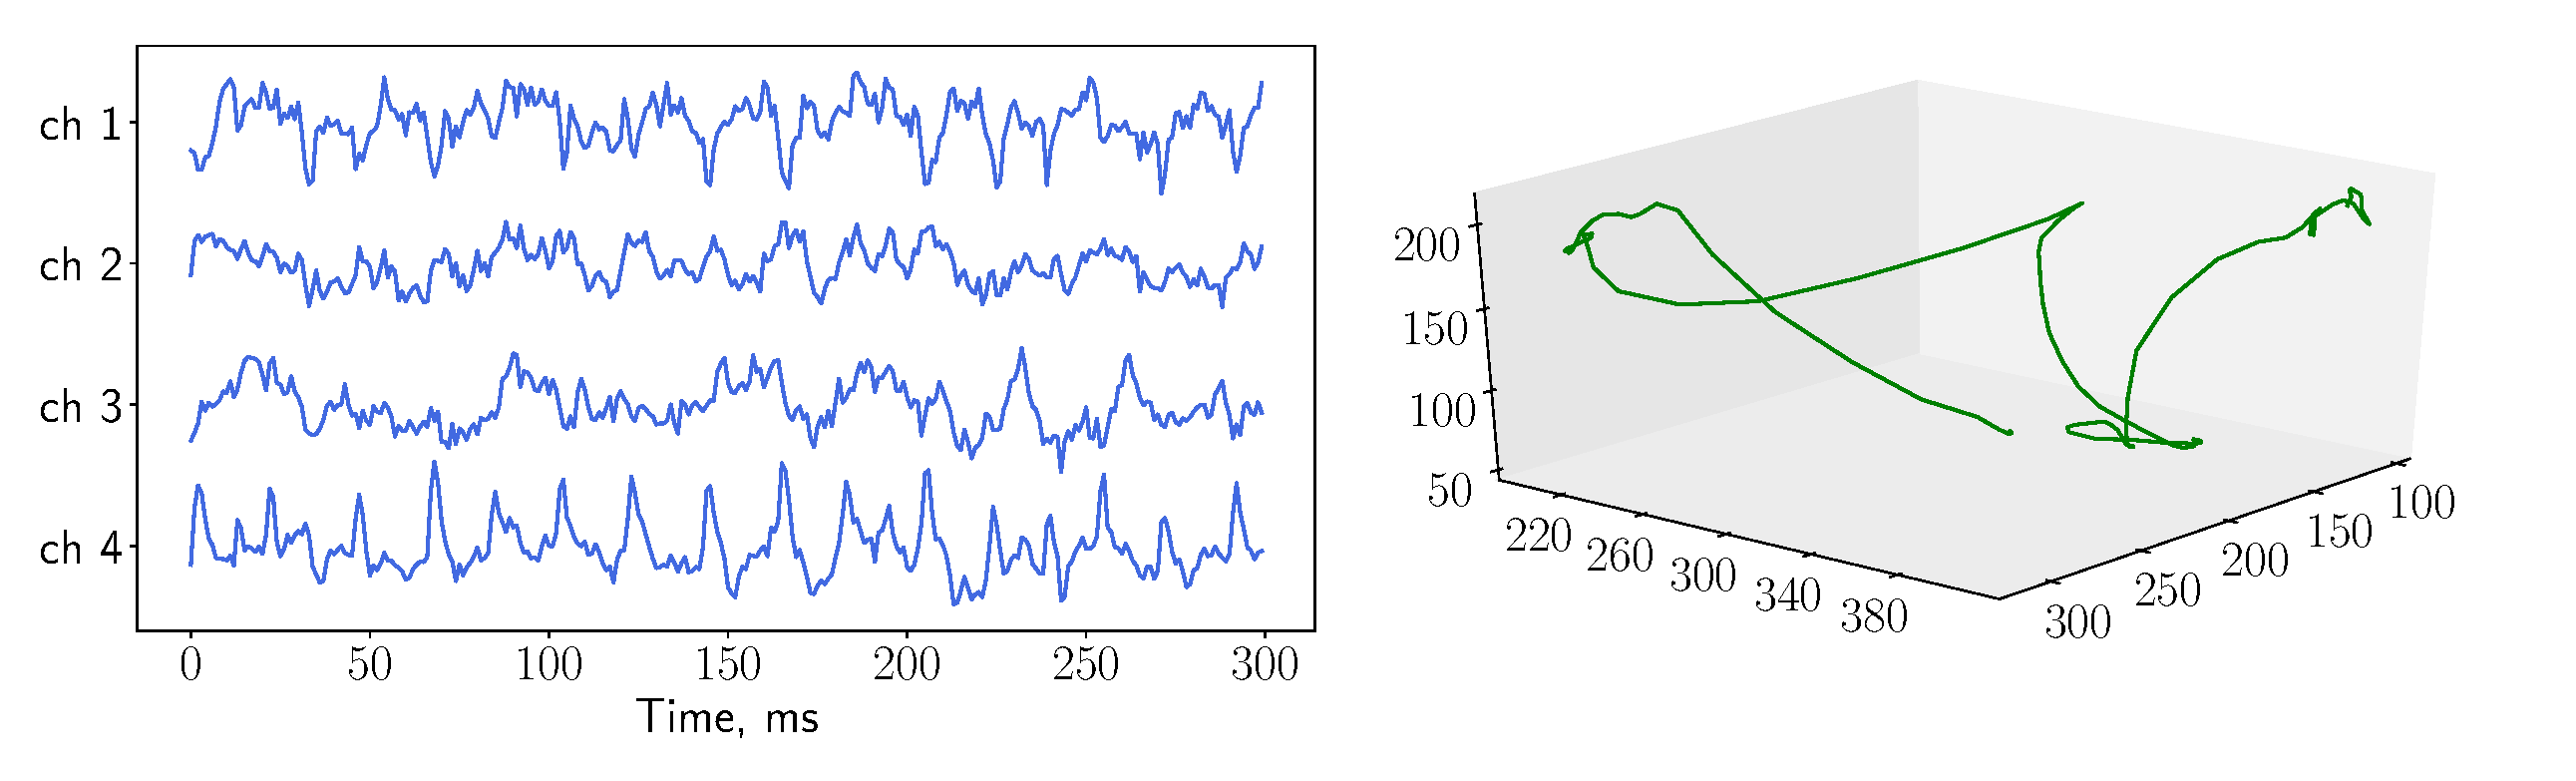
\includegraphics[width=\linewidth]{figs/ch2/ecog_data}
	\caption{Сигналы мозга (левый график) и 3D координаты руки (правый график)}
	\label{ch1:fig:ecog_data}
\end{figure}

Введём среднеквадратичную ошибку для некоторых матриц $\mathbf{A} = [a_{ij}]$ и $\mathbf{B} = [b_{ij}]$
\[
\text{MSE} (\mathbf{A}, \mathbf{B}) = \sum_{i,j} (a_{ij} - b_{ij})^2.
\]
Для оценивания качества аппроксимации вычисляется значение нормированной среднеквадратичной ошибки
\begin{equation}
\text{NMSE}(\bY,  \mathbf{\hat{Y}}) = \frac{\text{MSE} (\bY, \mathbf{\hat{Y}})}{\text{MSE} (\bY, \mathbf{\bar{Y}})},
\label{ch1:eq:nmse}
\end{equation}
где $\mathbf{\hat{Y}}$~--- прогноз модели, $\mathbf{\bar{Y}}$~--- константный прогноз средним значением по столбцам матрицы.

\textbf{Результаты на данных электроэнергии.}
Для нахождения оптимальной размерности $l$ латентного пространства все данные потребления электроэнергии были разбиты на обучающую и валидационную части. 
Обучающая выборка состоит из $700$ объектов, валидационная из $370$. Зависимость нормированной квадратичной ошибки~\eqref{ch1:eq:nmse} от размерности $l$ латентного пространства представлена на Рис.~\ref{ch1:fig:energy_n_comp}. 
Сначала ошибка резко падает при увеличении размерности скрытого пространства, а затем стабилизируется.

\begin{figure}[ht]
	\centering
	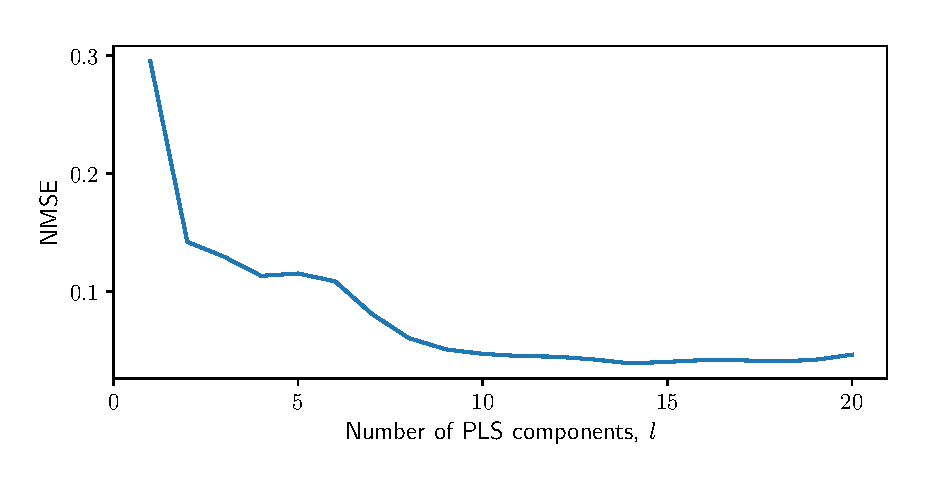
\includegraphics[width=0.75\linewidth]{figs/ch1/energy_n_comp}
	\caption{Прогноз потребления электроэнергии алгоритмом PLS при размерности латентного пространства $l$=14}
	\label{ch1:fig:energy_n_comp}
\end{figure}

Минимальная ошибка наблюдается при $l=14$. 
Построим прогноз потребления электроэнергии при данном $l$. 
Результат аппроксимации изображен на Рис.~\ref{ch1:fig:energy_prediction}. Алгоритм PLS восстановил авторегрессионную зависимость и обнаружил дневную сезонность.

\begin{figure}[ht]
	\centering
	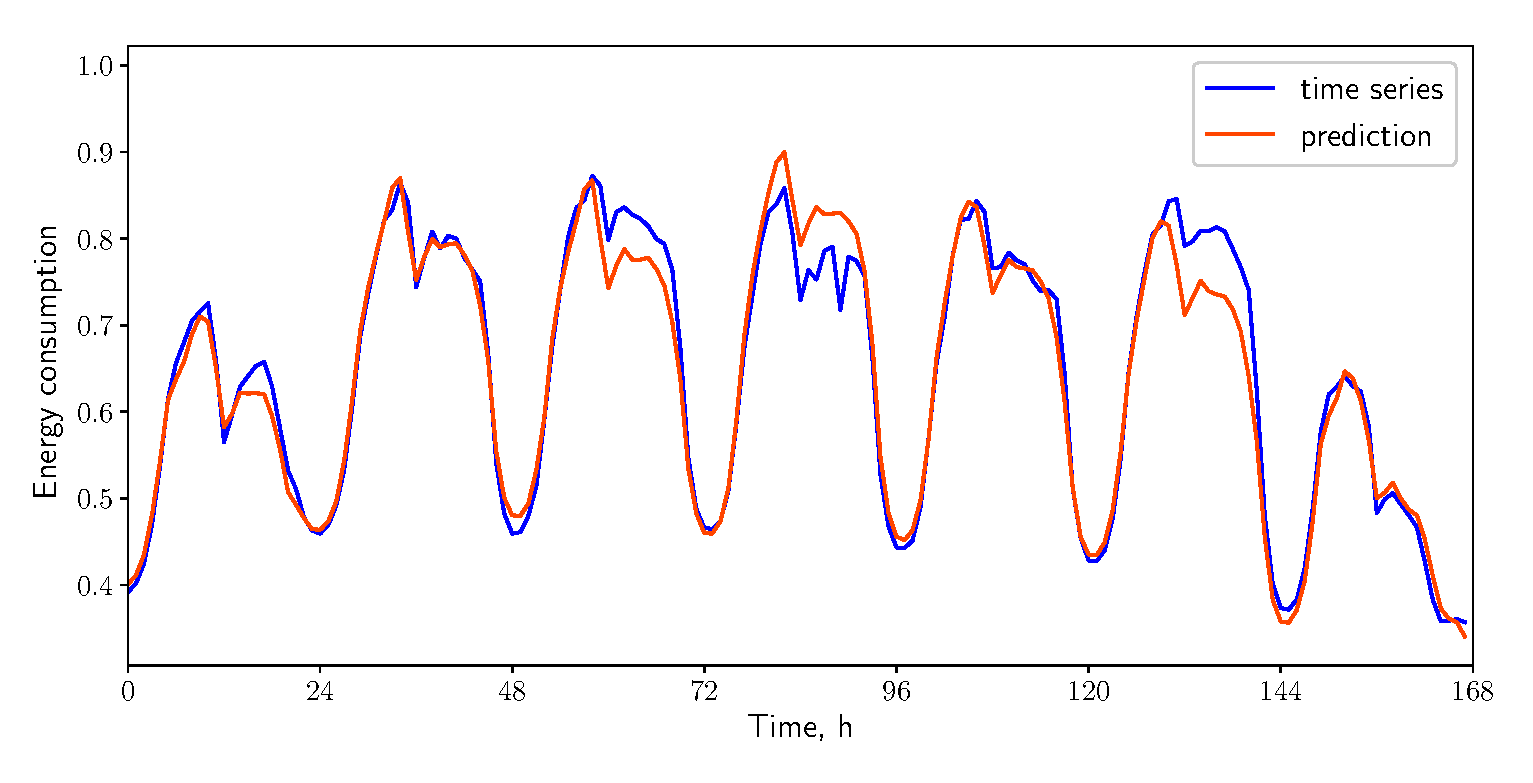
\includegraphics[width=0.95\textwidth]{figs/ch1/energy_prediction}
	\caption{Зависимость ошибки от размерности латентного пространства для данных потребления электроэнергии}
	\label{ch1:fig:energy_prediction}
\end{figure}

\textbf{Результаты на данных электрокортикограммы.}
На Рис.~\ref{ch1:fig:ecog_n_comp} представлена зависимость нормированной квадратичной ошибки~\eqref{ch1:eq:nmse} от размерности латентного пространства. Ошибка аппроксимации меняется незначительно при $l > 5$.
Таким образом совместное описание пространственно-временного спектрального представления объектов и пространственного положения руки может быть представлено вектором размерности $l \ll n$.
Зафиксируем $l = 5$. 
Пример аппроксимации положения руки изображен на Рис.~\ref{ch1:fig:ecog_prediction}. 
Сплошными линиями изображены истинные координаты руки по всем осям, пунктирными линиями показана аппроксимация методом PLS.
 
\begin{figure}[ht]
	\centering
	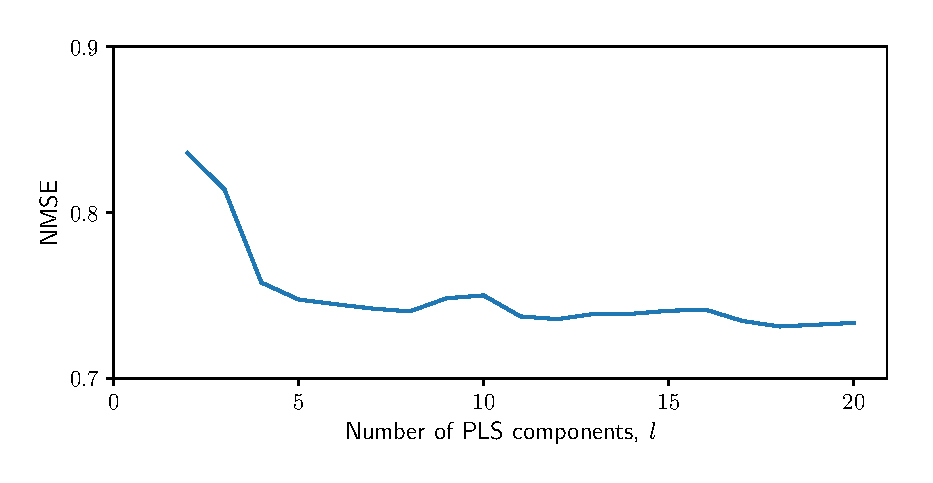
\includegraphics[width=0.75\linewidth]{figs/ch1/ecog_n_comp}	
	\caption{Зависимость ошибки от размерности латентного пространства для данных ECoG}
	\label{ch1:fig:ecog_n_comp}
\end{figure}

\begin{figure}[ht]
	\centering
	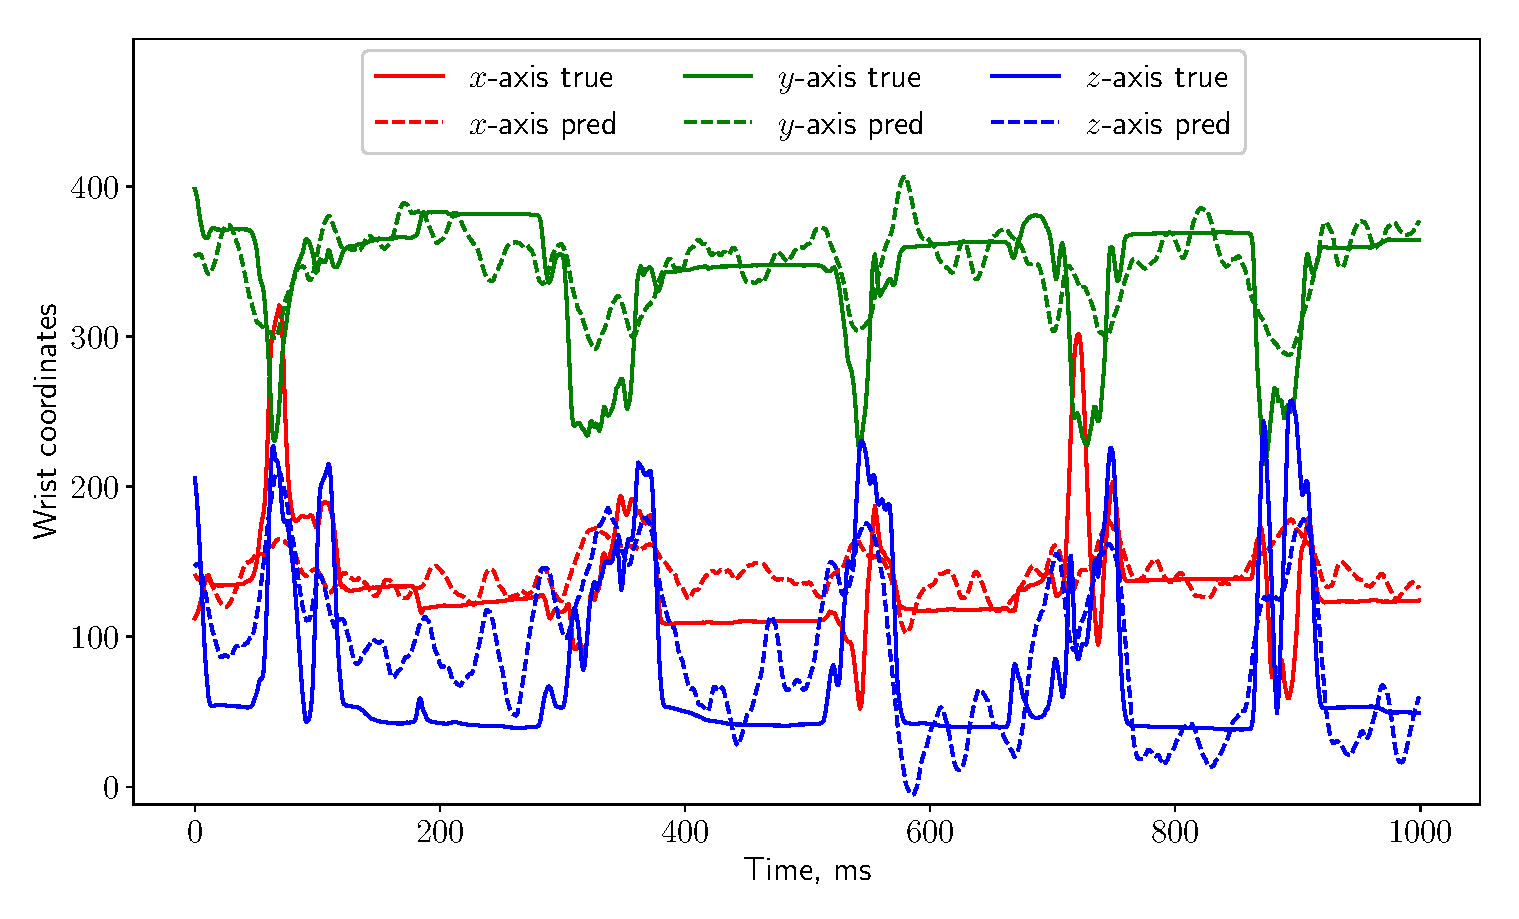
\includegraphics[width=\textwidth]{figs/ch1/ecog_prediction}
	\caption{Прогноз движения руки по данным ECoG алгоритмом PLS при размерности латентного пространства $l=5$}
	\label{ch1:fig:ecog_prediction}
\end{figure}

\section{Анализ нелинейных зависимостей проекций в скрытое пространство}
Цель вычислительного эксперимента~-- сравнительный анализ рассматриваемых моделей.
Рассматриваются данные, для которых сложность класса линейных методов неадекватно низка.
Нелинейные модели позволяют получить точный прогноз при адекватной сложности.
В рамках вычислительного эксперимента написан программный комплекс для решения поставленных задач~\cite{source_code}.

\begin{figure}[!tp]
\centering 
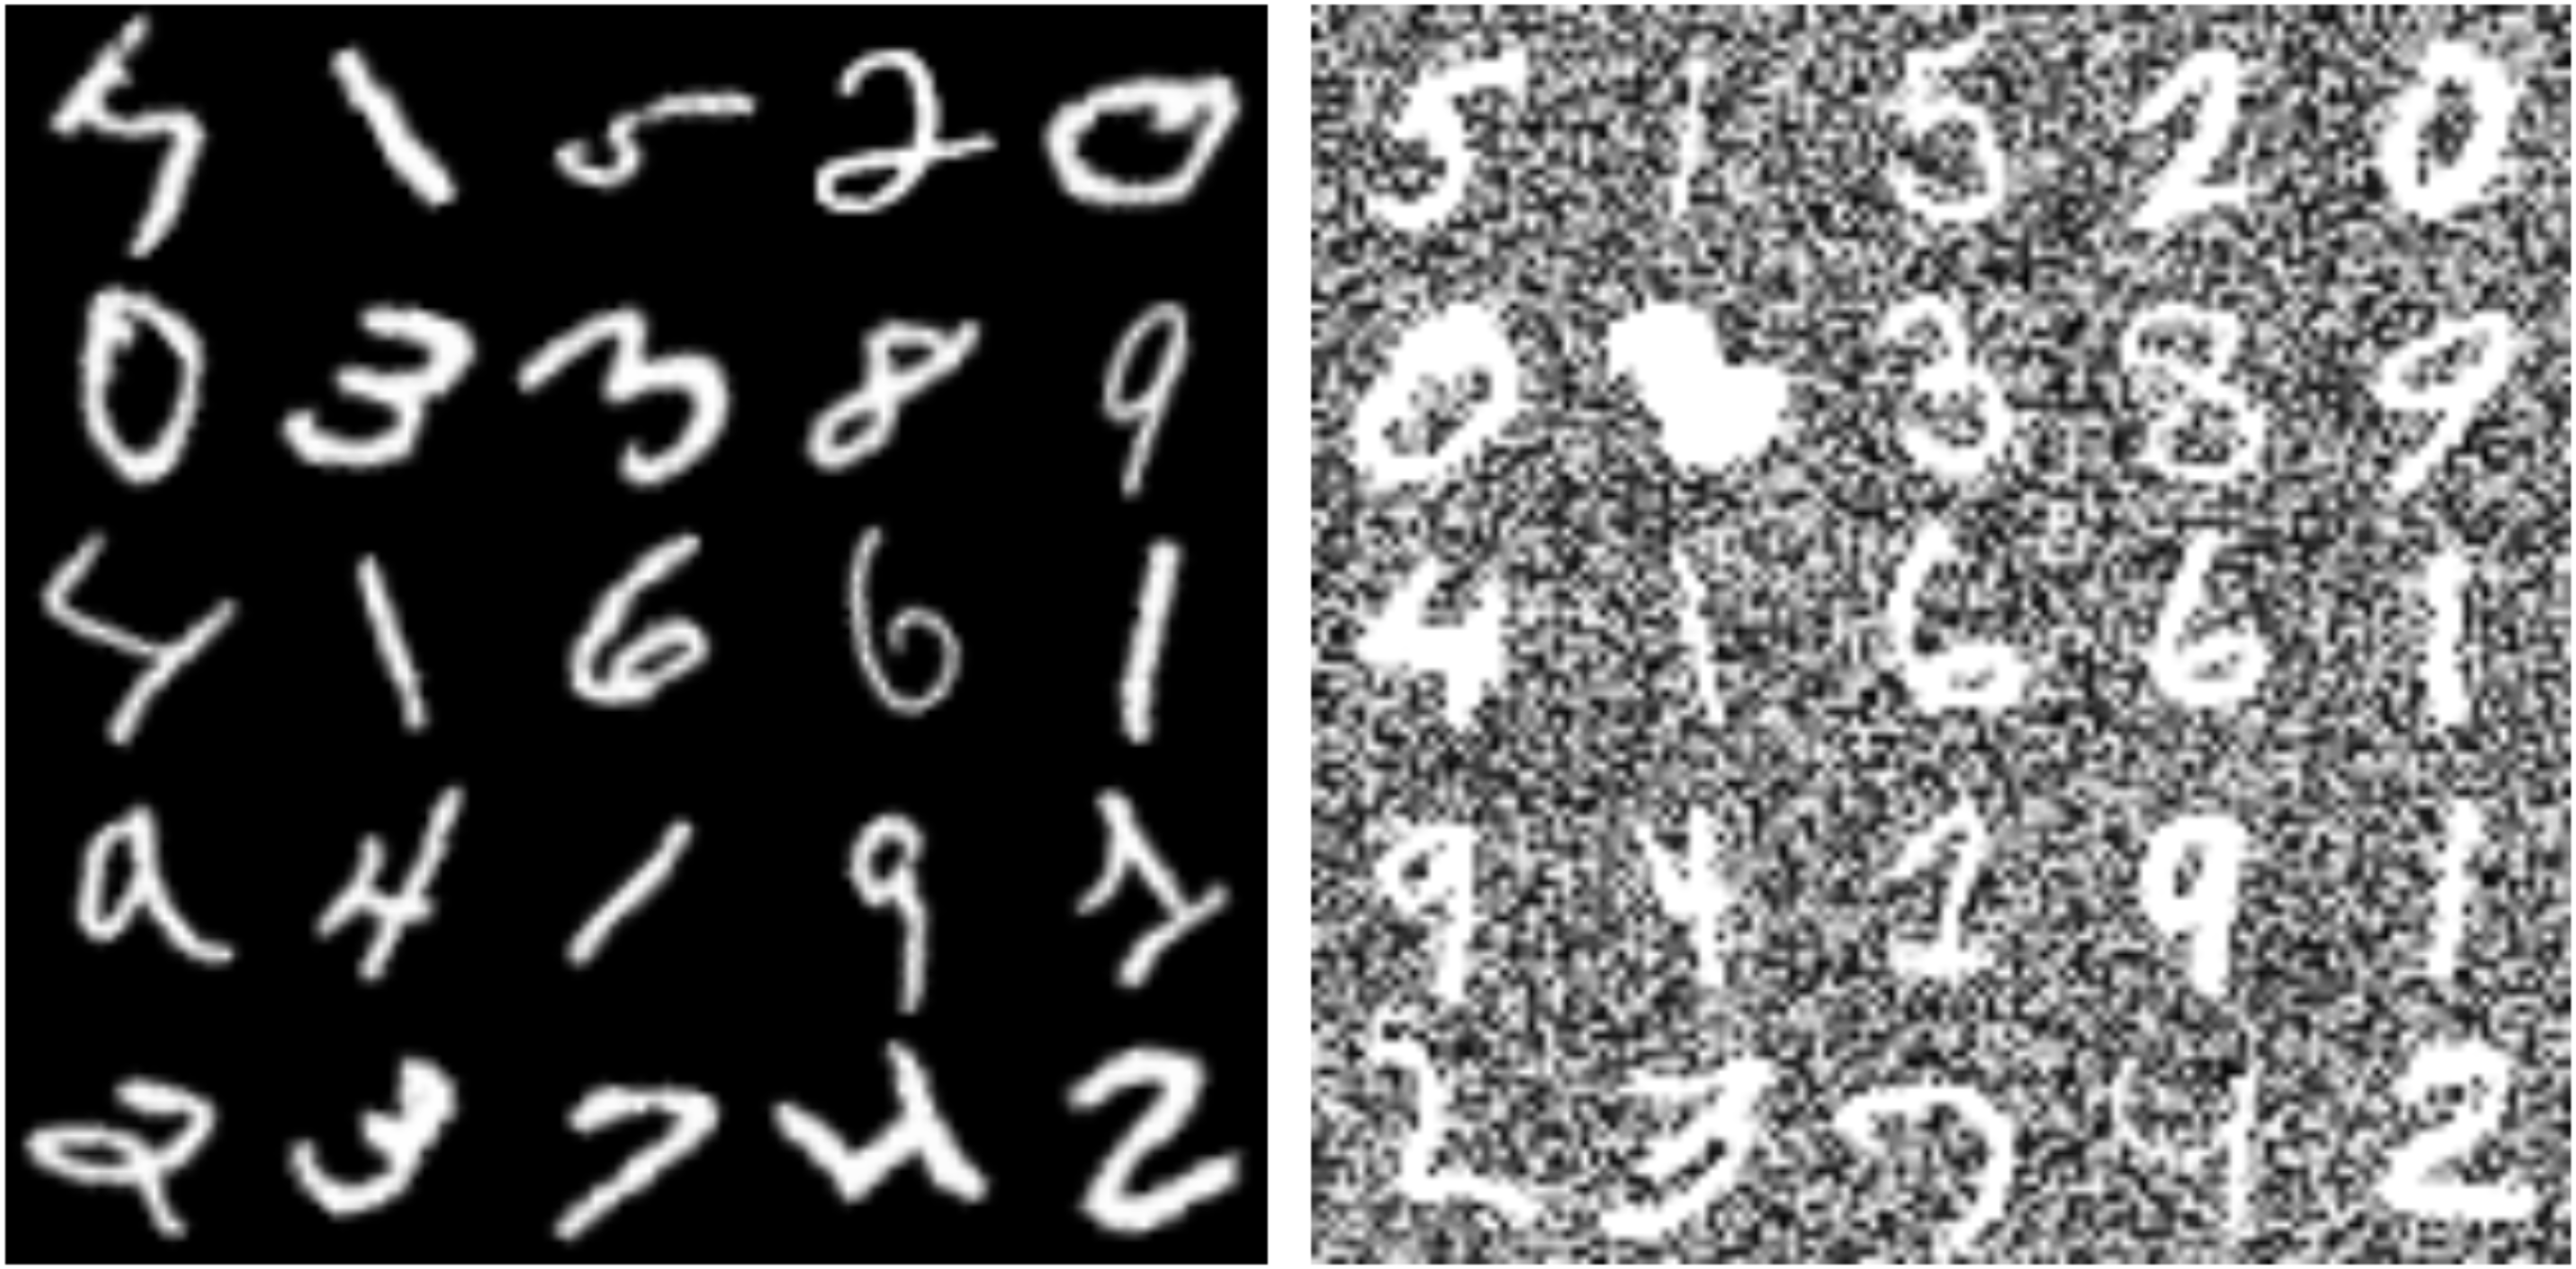
\includegraphics[width=\linewidth]{figs/ch2/noisy_mnist}
\caption{Зашумленные изображения из набора данных MNIST}
\label{fgr:1}
\end{figure}

\textbf{Задача фильтрации шума}

Проведем сравнение качества Deep CCA и CCA на задаче классификации зашумленных цифровых изображений, представленных на рис.~1. Для этого используется набор данных MNIST~\cite{MNIST}, который состоит из 70\,000 цифровых изображений $28 \times 28$ образцов рукописного написания цифр. Предлагается получить два новых набора данных $\bX$ и $\bY$ следующим образом. Первый набор получается поворотом исходных изображений на угол в диапазоне $[\frac{-\pi}{4}, \frac{\pi}{4}]$. Для получения второго набора данных для каждой картинки из первого набора данных ставится в соответствие случайным образом картинка с той же цифрой, но с добавлением независимого случайного шума, распределенного равномерно на отрезке $[0,1]$.

\begin{table}[!bp]
\caption{Точность классификации линейного SVM для алгоритмов Deep CCA и CCA}
\centering
\begin{tabular}{l|cc}
\hline
	Скользящий контроль & Deep CCA ($L=3$) & CCA \\  \hline
	Валидация & 92,74\%  &  76,21\%\\
	Тест & 92,14\% & 76,07\% \\
	\hline
\end{tabular}
\label{tbl:1}
\end{table}

Применив к двум новым наборам данных DeepCCA или CCA, получаем новое низкоразмерное признаковое пространство, которое игнорирует шумы в исходных данных. Таким образом, получаем функции кодирования $\varphi_1$ и $\psi_1$ для исходных наборов данных. На новых признаках, полученных разными моделями (DeepCCA и CCA), для первого набора данных, то есть на данных после применения функции кодирования $\varphi_1$ к первому набору исходных данных, обучим линейный SVM-классификатор. Показателем эффективности будет точность классификации линейного SVM на тестовых данных. В случае построения адекватного скрытого пространства полученные образы объектов будут линейно разделимы. Результаты эксперимента приведены в табл.~\ref{tbl:1}. Модель Deep CCA представляет собой нейронную сеть с $L=3$ скрытыми слоями. Точность классификации нелинейной модели существенно выше линейного алгоритма CCA.

\textbf{Задача восстановления изображений}
Для анализа процедуры согласования проведен вычислительный эксперимент с предложенными нелинейными моделями.
Для снижения размерности пространства используются нейросетевые модели автокодировщика c согласованием скрытого пространства~\eqref{concordance}.
В качестве базовых моделей используются модель автокодировщика без согласования скрытых пространств, а также линейный PLS. В качестве исходного набора данных используется набор данных MNIST~\cite{MNIST}. Каждое изображение поделено на левую и правую части, как показано на рис.~\ref{fgr:3}. Модель по левому изображению восстанавливает правое изображение.

\begin{figure}[!tp]
\centering 
\includegraphics[width=\linewidth]{figs/ch2/left_right_mnist}
\caption{Набор данных MNIST, в котором каждое изображение разделено пополам}
\label{fgr:3}
\end{figure}

Модель EncNet1~--- нейронная сеть с нелинейными функциями активации, которая обучается на данных после преобразования их автоэнкодером. Модель LinNet1~--- нейронная сеть с одним линейным слоем, которая также обучается на преобразованных данных. Для EncNet1 и LinNet1 автоэнкодеры для объектов и ответов используют совместную функцию потерь, которая связывает выходы энкодеров. Модели EncNet2 и LinNet2 устроены аналогично EncNet1 и LinNet1 соответственно, но в автоэнкодерах нет совместной функции потерь. Модель DumbNet~---  нейронная сеть, которая обучается на исходных данных и имеет такую же структуру, что и EncNet, то есть имеет такое же число слоев и в каждом слое такое же количество нейронов, что и у EncNet.

\begin{table}[!bp]
\caption{Квадратичная ошибка для нелинейных моделей в задаче восстановления правой части изображения по левой}
\centering
\begin{tabular}{l|cccccc}
\hline
	& EncNet1 & LinNet1 & EncNet2 & LinNet2 & DumbNet & PLS\\  \hline
	Число параметров, тыс. & 283 & 239 & 283 & 239  & 283 & --\\
	Ошибка на тесте & 0,147 & 0,235 & 0,149 & 0,236 & 0,128 & 0,188 \\
	\hline
\end{tabular}
\label{tbl:2}
\end{table}

Для оценки качества моделей вычислялась среднеквадратичная ошибка. Примеры восстановленных изображений показаны на рис.~\ref{fgr:2}. Качество моделей, а также их сложность представлены в табл.~\ref{tbl:2}.
На рис.~\ref{fgr:2} продемонстрировано, что предложенные модели EncNet и LinNet позволяют получить более четкие и различимые изображения, в отличие от базовой нелинейной модели DumbNet и линейной модели PLS.
Несмотря на заметное улучшение визуального качества изображений, ошибка предложенных моделей выше, чем у модели DumbNet.
Авторы предполагают, что это связано с тем, что среднеквадратичная ошибка оказалась неадекватной метрикой в пространстве изображений.
Нахождение оптимальной метрики для оценки качества предложенных алгоритмов может быть одним из возможных направлений развития текущей работы.

\begin{figure}[!tp]
\centering 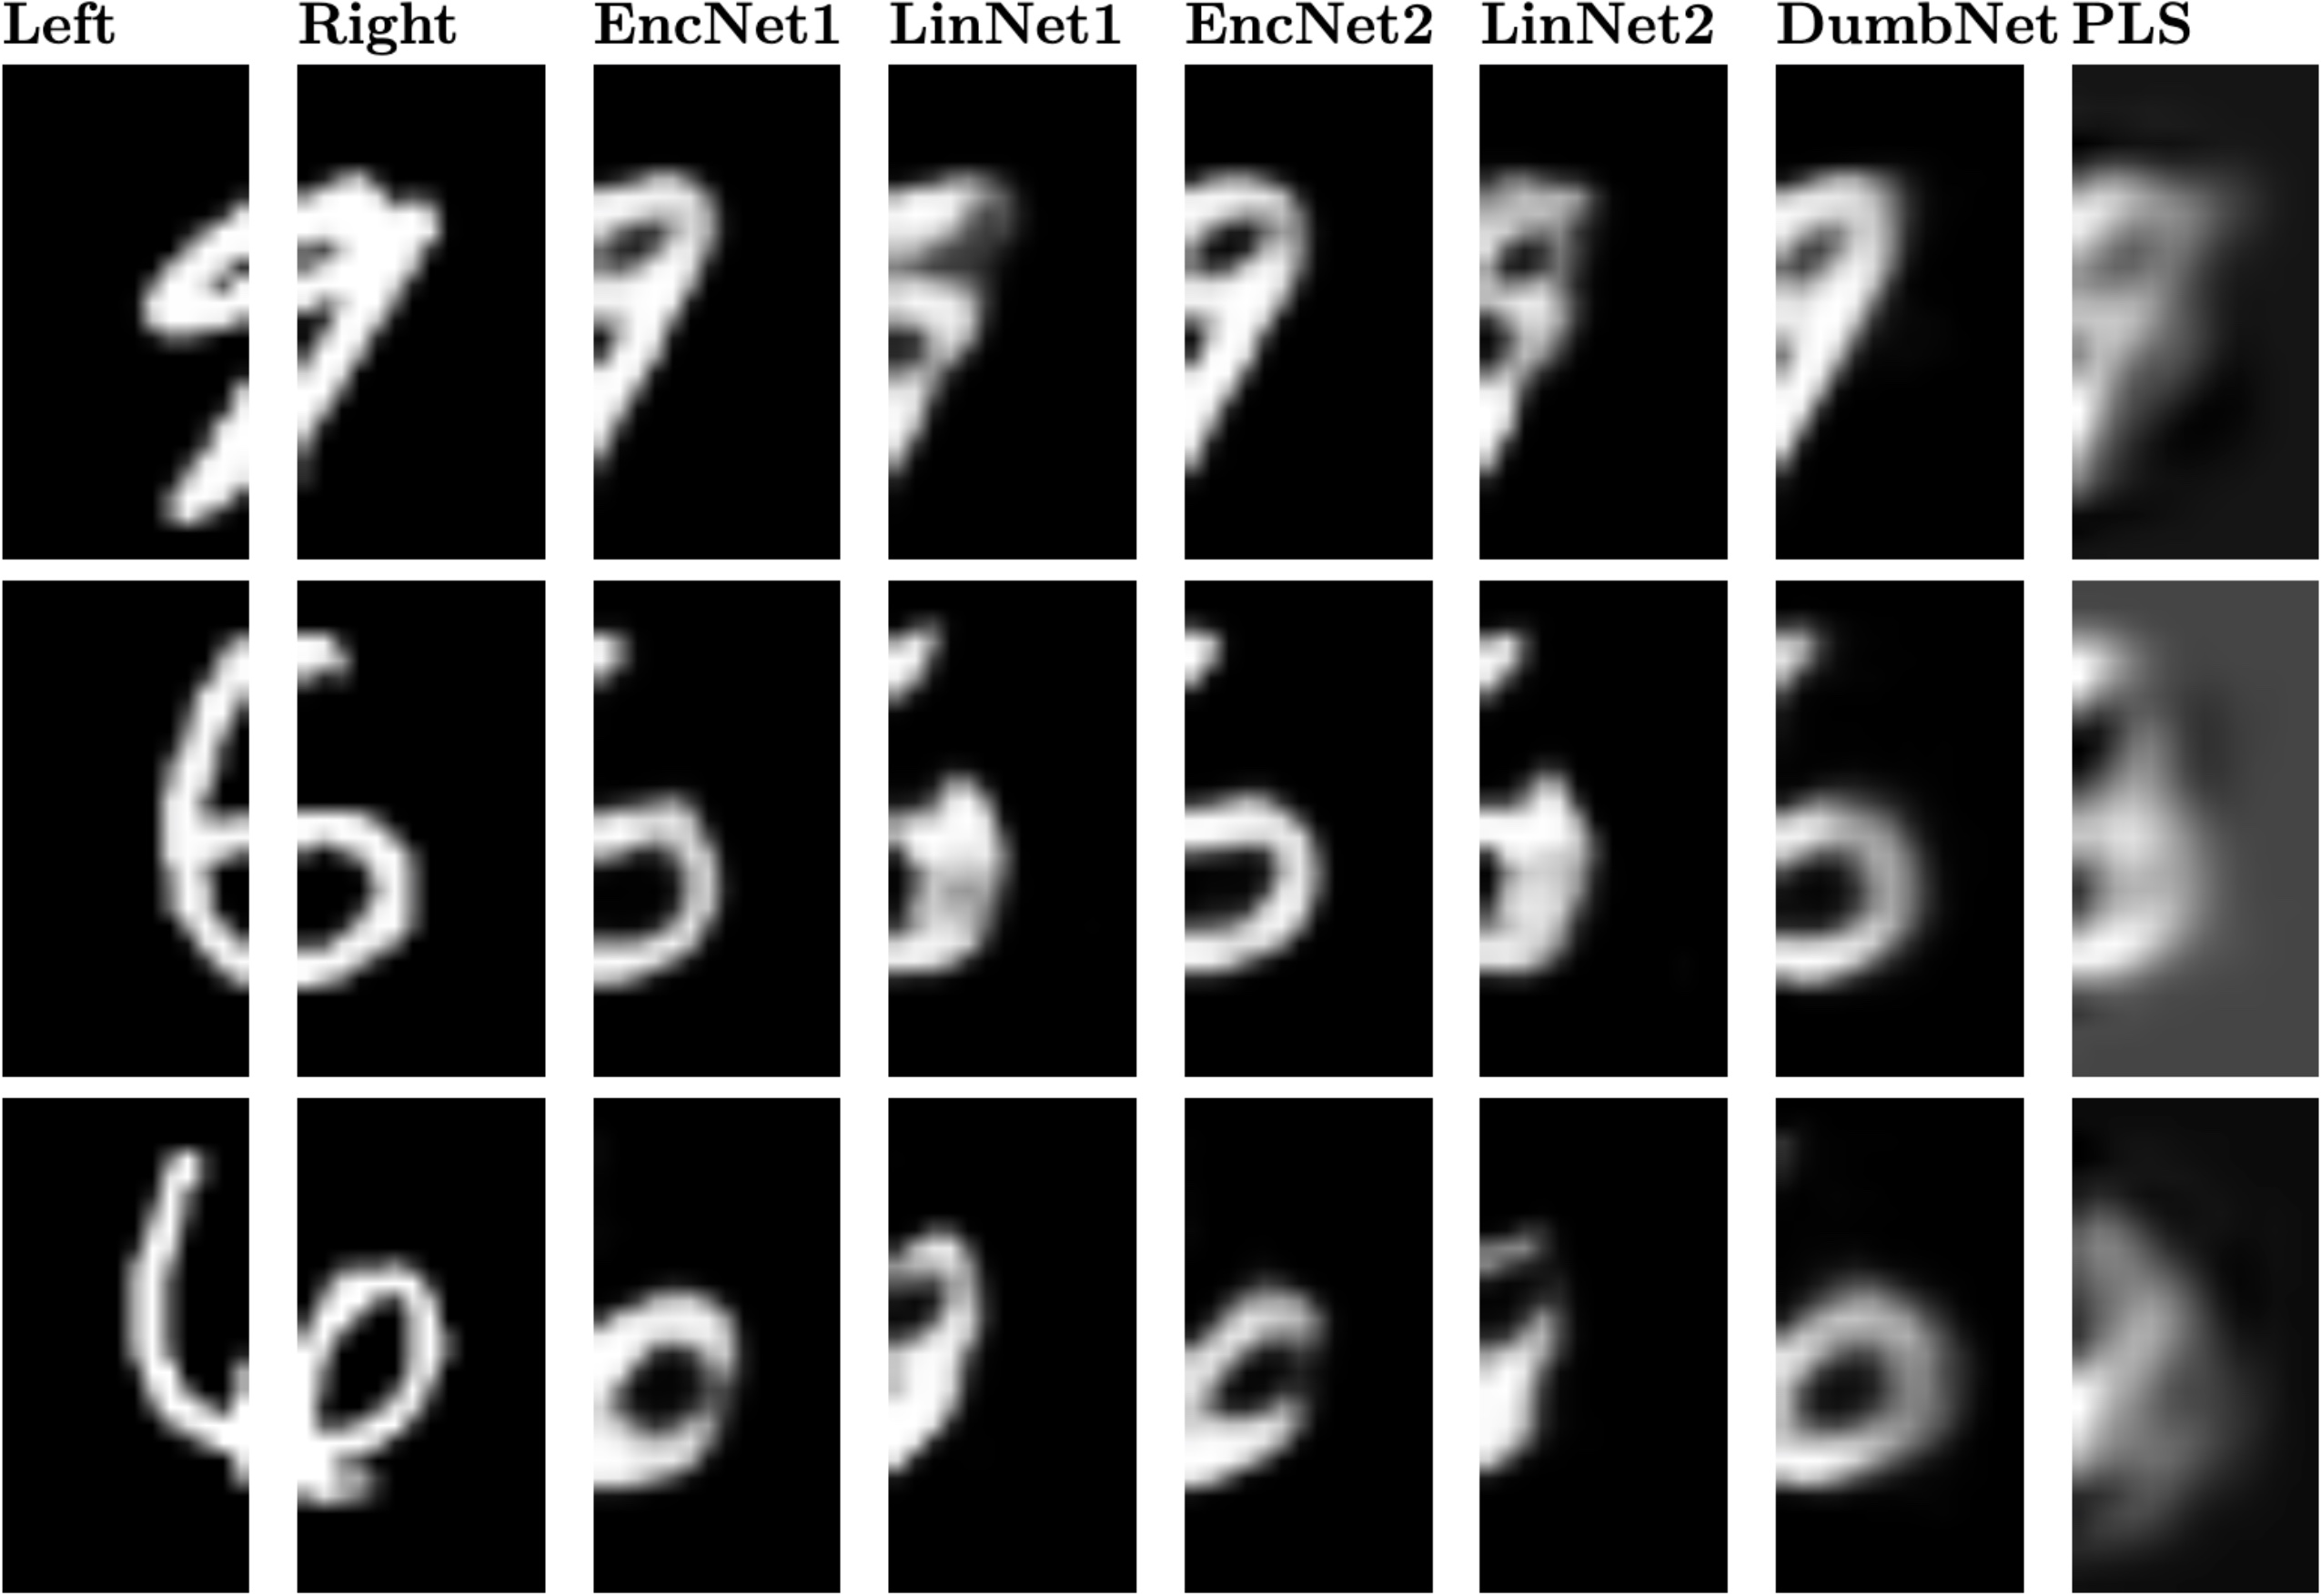
\includegraphics[width=\linewidth]{figs/ch2/mnist_preds}
\caption{Пример реконструкции правой части изображения по левой для рассматриваемых моделей}
\label{fgr:2}
\end{figure}
